\documentclass[30pt]{report}
%\documentclass[12pt,twoside]{report}
\usepackage[utf8]{inputenc}
%\usepackage{amsmath}
%\usepackage{amsfonts}
%\usepackage{amssymb}
\usepackage{float}
\usepackage{caption}
\usepackage{subcaption}
\usepackage{graphicx}
\graphicspath{ {Images/} }
\usepackage{xcolor}
\usepackage{listings}
\usepackage{multirow}
\usepackage[bottom=0.5in,margin=1in,footskip=0.4in, headsep=.2in]{geometry}
\usepackage{longtable}
%\usepackage{hyperref}
\usepackage{sectsty}
\usepackage{url}
\usepackage{array}
\usepackage{xcolor,colortbl}% http://ctan.org/pkg/xcolor
\usepackage{amssymb}
%\usepackage{geometry}

\newcommand{\done}{\cellcolor{green}}  %{0.9}
\newcommand{\hcya}[1]{{\cellcolor{yellow} #1}}
\newcommand{\hcy}[1]{{\cellcolor{orange} #1}}
\newcommand{\hcyan}[1]{{\cellcolor{red} #1}}
\newcommand{\hc}[1]{{\cellcolor{blue} #1}}

\newcommand{\package}[1]{ \texttt{ \textbf{#1}}}

\newcommand{\server}[1]{ \textit{#1}}


\newcommand{\file}[1]{  \texttt{ \textit{#1}}}
\newcommand{\unit}[1]{ \textrm{#1}}
\newcommand{\constant}[1]{ \textrm{\textit{#1}}}
\newcommand{\component}[1]{  \texttt{#1}}
\newcommand{\sensor}[1]{  \textit{#1}}
\newcommand{\option}[1]{  \texttt{#1}}
%\newcommand{\output}[1]{  \texttt{#1}}

%\lstdefinestyle{DOS}
%{
%	backgroundcolor=\color{white},
%	basicstyle=\scriptsize\color{black}\ttfamily,
%	xleftmargin=\parindent
%	%	basicstyle=\ttfamily,
%	%	keywordstyle=\bfseries,
%	%	showstringspaces=false,
%	%	morekeywords={include, printf}
%}

\lstdefinestyle{DOS}
{
	backgroundcolor=\color{gray},
	basicstyle=\scriptsize\color{black}\ttfamily,
	xleftmargin=\parindent
	%	basicstyle=\ttfamily,
	%	keywordstyle=\bfseries,
	%	showstringspaces=false,
	%	morekeywords={include, printf}
}
\author{Authors:  Telescope Operators}
\date{}


\begin{document}
%	\maketitle
{\huge
\noindent
\LaTeX\  template for Meerkat Telescope Operator Manual
	
\noindent
\section*{Goals:}
\begin{itemize}
  \item To prepare the manual for printing.
  
  \item To create a platform that can handle professional and high quality document as required in scientific reporting.
\end{itemize}
  
\noindent  
\section*{Advantages of Latex over Word:}
\begin{itemize}
   \item Handles large documents and Graphics 
   \item Text quaity and layout far better that word.
   \item  Complex Mathamatical equations and scientific features
    \item  Better referencing.
    \item Version control possible 
\end{itemize}  
\section*{Disadvatages:}
\begin{itemize}
   \item   \LaTeX\ is typesetting/programming language, needs time to learn.
   \item  Commands must be typed in.
  \item   Errors due incompatable packages.
\end{itemize}  
\noindent   
 \section*{Getting Started with Latex}
 \begin{itemize} 
 	
   \item Install \LaTeX\ compiler (MiTex for Windows, MacTex for Mac, TexLive for linux/Unix )
   \item Install Latex Tex editor ( TexMaker, TexStudio, etc )
   \item Or \textbf{Overleaf} for cloud typesetting.
   


   
\end{itemize}
   
\section*{Elements of the Manual that were typeset}

\begin{itemize} 
\item All figures (more than 130) must be:	
\begin{itemize} 
	\item referenced 
	\item captioned
	\item size scaled 
	\item clear - not blury (latex has some tools to improve the quality of images.) 
\end{itemize}
\clearpage

An example of bad image is shown in 
\begin{figure}[H]
	\centering
	%\includegraphicsdpi{100}{}{bur1.png}     
	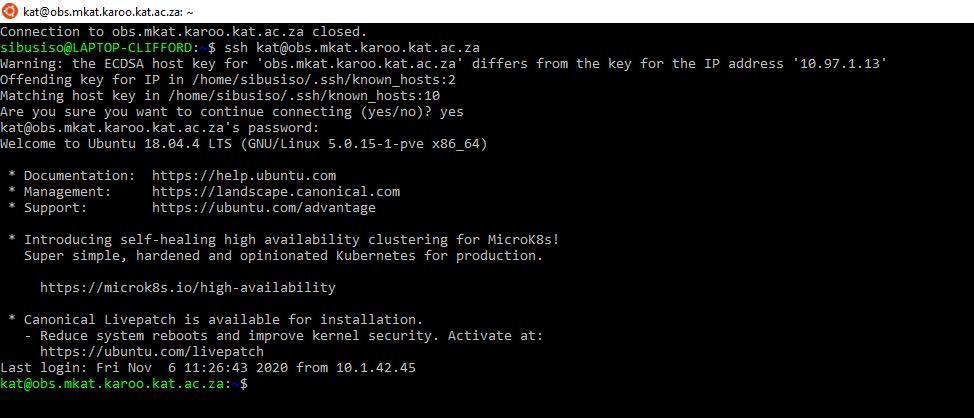
\includegraphics[scale=0.43]{image87.png}
	
	%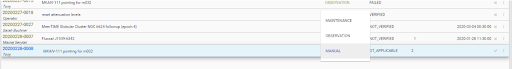
\includegraphics[resolution=100]{bur1.png}
	\caption{Linus add vpn dialog box}
	\label{fig:image87}
\end{figure}
\begin{figure}[H]
	\centering
	%\includegraphicsdpi{100}{}{bur1.png}     
	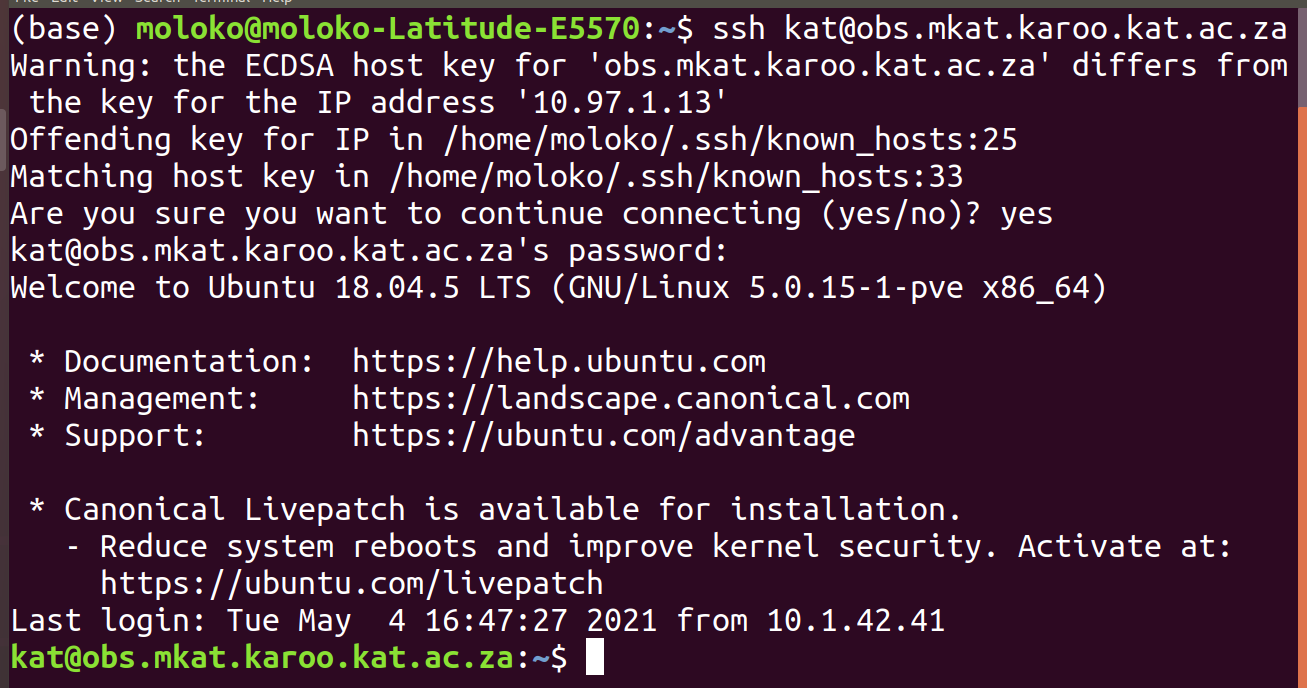
\includegraphics[scale=0.33]{terminal.png}
	
	%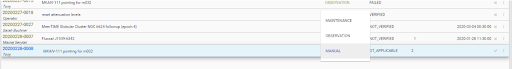
\includegraphics[resolution=100]{bur1.png}
	\caption{Good image}
	\label{fig:image2}
\end{figure}
\clearpage
\noindent
\item Bulleted lists and common errors:
 \begin{itemize} 
	
	\item[$\circ$]  consistant bulleted lists across the documnent
	\item[$\circ$]  add inroductory sentence to bulleted list.
	\item[$\circ$]  harmony between inroductory sentence and list
	\item[$\circ$]  Semi-colon or not?

\end{itemize}
\item Naming convections and typographycal styles:
\begin{itemize} 
	
	\item[$\circ$] SI units
	\item[$\circ$] Consistant font styles for code, Names of files, servers, software, links, etc. for example,
\begin{lstlisting}[style=DOS]
ssh kat@obs.mkat.karoo.kat.ac.za
ipython			
import katuilib
configure_cam("camcam","all")
\end{lstlisting}
		
\end{itemize}

\item Common technical errors: 
\begin{itemize} 
	
   \item[$\circ$]  incorrect use of punctuation, (i.e :, (), $-$ )
	\item[$\circ$] missing punctuation
	 \item[$\circ$] Language - UK vs US?
	
\end{itemize}


\end{itemize}

} 



	
\end{document}